In this section, results will be exposed that follow the previously explained methodology. They answer issues like project's size, project's development model, companies supporting development, and most valuable developers--contributors. For that matter, results will be categorized in repository-related, developers' mailing list-related and unassigned bugs' mailing list-related.    

\subsection{Repository}

In order to measure the repository size, a set of variables are taken into account: number of commits, number of committers, number of files under version control, number of lines of code and years of activity. Table \ref{repo:summary} presents that information. In figure \ref{sloccount:summary} the distribution of programming languages in the project is shown\footnote{Number of lines of code and programming language distribution were generated using David A. Wheeler's `SLOCCount'.}.	

\begin{table}[ht]
\begin{center}
\begin{tabular}{lr}
  \hline
 Concept & Count \\ 
  \hline
Number of commits & 44143 \\ 
Number of committers & 195 \\
Number of files under version control & 80860\\
Number of lines & 824955\\
Years of activity & 9\\
   \hline
\end{tabular}
\caption{Brief summary of the repository's activity}
\label{repo:summary}
\end{center}
\end{table}

\begin{figure}[!hptb]
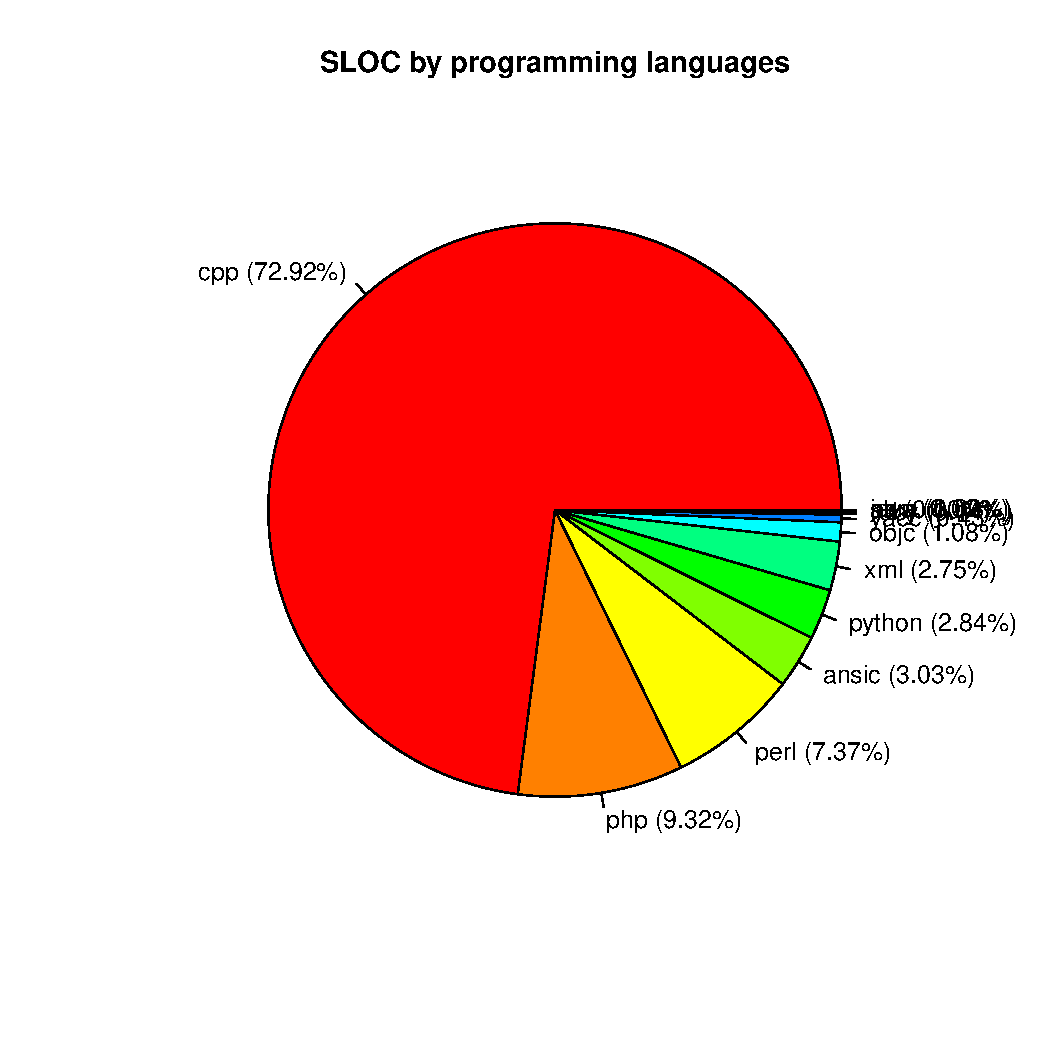
\includegraphics[width=400pt]{images/sloc.pdf}
\caption{Programming language distribution}
\label{sloccount:summary}
\end{figure}

Having presented the data about the project size, the following results will help identify the most important committers. Table \ref{commits:top20} shows the {\it All-time} top 20 committers. However, a quick glance at it lets us find several committers sharing their username, but using different email addresses. Results from table \ref{commits:top20grouped} show that information corrected, so users get their contribution added up even if they have used different email addresses to commit. We can identify one user, ``\textbf{darin}'', as the one who has done the most commits: $4876$.

% latex table generated in R 2.9.2 by xtable 1.5-6 package
% Wed Jan 20 20:01:11 2010
\begin{table}[!htpb]
\begin{center}
\begin{tabular}{rlr}
  \hline
 & Committer & Commit count \\ 
  \hline
1 & darin & 3583 \\ 
  2 & hyatt & 2158 \\ 
  3 & eric@webkit.org & 1967 \\ 
  4 & mjs & 1620 \\ 
  5 & hausmann@webkit.org & 1174 \\ 
  6 & rjw & 1104 \\ 
  7 & darin@apple.com & 1076 \\ 
  8 & kocienda & 958 \\ 
  9 & mitz@apple.com & 945 \\ 
  10 & mrowe@apple.com & 941 \\ 
   \hline
\end{tabular}
\caption{Top 10 committers. Multiple accounts ignored}
\label{commits:top20}
\end{center}
\end{table}

% latex table generated in R 2.9.2 by xtable 1.5-6 package
% Wed Jan 20 20:01:11 2010
\begin{table}[!htpb]
\begin{center}
\begin{tabular}{rlr}
  \hline
 & Committer & Commit count \\ 
  \hline
1 & darin & 4876 \\ 
  2 & hyatt & 3042 \\ 
  3 & eric & 1967 \\ 
  4 & mjs & 1842 \\ 
  5 & hausmann & 1417 \\ 
  6 & andersca & 1376 \\ 
  7 & ggaren & 1287 \\ 
  8 & weinig & 1263 \\ 
  9 & ap & 1252 \\ 
  10 & aroben & 1164 \\ 
   \hline
\end{tabular}
\caption{Top 10 committers. Multiple accounts grouped}
\label{commits:top20grouped}
\end{center}
\end{table}


% Si se desea introducir el modelo de cebolla, correspondería aquí.

In order to have information about last trends, last year top 20 committers are shown in table \ref{commits:2009top20}. Our previously identified {\it top committer}, ``darin'', is now located at the $5^{th}$ place, being ``eric@webkit.org'' the developer who has done the biggest amount of commits last year: $1646$. His progression is worth noting, as he was ranked $3^{rd}$ all-time, with $1967$ commits, which means he has done  $83,68\%$ of his work last year.

% latex table generated in R 2.9.2 by xtable 1.5-6 package
% Wed Jan 20 20:01:11 2010
\begin{table}[!htpb]
\begin{center}
\begin{tabular}{rlr}
  \hline
 & Committer & Commit count \\ 
  \hline
1 & eric@webkit.org & 1646 \\ 
  2 & abarth@webkit.org & 474 \\ 
  3 & hausmann@webkit.org & 440 \\ 
  4 & kov@webkit.org & 387 \\ 
  5 & darin@apple.com & 385 \\ 
  6 & mrowe@apple.com & 364 \\ 
  7 & simon.fraser@apple.com & 357 \\ 
  8 & mitz@apple.com & 334 \\ 
  9 & hyatt@apple.com & 322 \\ 
  10 & oliver@apple.com & 320 \\ 
   \hline
\end{tabular}
\caption{Top 10 committers during 2009}
\label{commits:2009top20}
\end{center}
\end{table}


Complete email addresses are presented in table \ref{commits:2009top20}. After November 2007, users committing to the repository stopped using just their username, and started using an email address for commits. Table \ref{commits:november} shows who did the last commits using the old username schema, and how after day 12 nobody used the username alone.

% latex table generated in R 2.9.2 by xtable 1.5-6 package
% Wed Jan 20 20:01:11 2010
\begin{table}[!htpb]
\begin{center}
\begin{tabular}{rlllr}
  \hline
 & Committer & First contribution & Last contribution & Commit count \\ 
  \hline
1 & hausmann & 2007-11-07 11:32:07 & 2007-11-10 23:24:34 &  77 \\ 
  2 & aroben & 2007-11-01 02:22:35 & 2007-11-08 00:45:58 &  20 \\ 
  3 & antti & 2007-11-03 01:23:43 & 2007-11-12 02:54:55 &  14 \\ 
  4 & alp & 2007-11-01 19:37:36 & 2007-11-06 03:53:16 &  11 \\ 
  5 & oliver & 2007-11-02 00:30:25 & 2007-11-12 09:00:29 &  11 \\ 
  6 & eseidel & 2007-11-06 05:55:25 & 2007-11-12 01:34:37 &  10 \\ 
  7 & kmccullo & 2007-11-01 01:06:56 & 2007-11-09 09:29:20 &  10 \\ 
  8 & kevino & 2007-11-01 22:36:00 & 2007-11-06 07:39:22 &   9 \\ 
  9 & mjs & 2007-11-01 06:02:30 & 2007-11-07 08:23:25 &   9 \\ 
  10 & ddkilzer & 2007-11-03 07:58:34 & 2007-11-07 22:54:57 &   7 \\ 
  11 & sfalken & 2007-11-08 08:40:08 & 2007-11-09 18:16:39 &   7 \\ 
  12 & ap & 2007-11-01 10:21:30 & 2007-11-06 19:10:22 &   7 \\ 
  13 & ggaren & 2007-11-01 09:36:58 & 2007-11-05 22:56:09 &   6 \\ 
  14 & weinig & 2007-11-01 22:33:33 & 2007-11-10 00:34:19 &   5 \\ 
  15 & tristan & 2007-11-05 23:43:45 & 2007-11-10 00:51:48 &   4 \\ 
  16 & justing & 2007-11-01 00:23:26 & 2007-11-07 02:13:47 &   4 \\ 
  17 & mitz & 2007-11-01 16:30:23 & 2007-11-02 07:27:29 &   3 \\ 
  18 & hyatt & 2007-11-01 04:05:41 & 2007-11-09 20:57:39 &   3 \\ 
  19 & adele & 2007-11-01 20:01:09 & 2007-11-06 20:53:18 &   3 \\ 
  20 & adachan & 2007-11-06 01:02:50 & 2007-11-06 03:10:05 &   2 \\ 
  21 & bdakin & 2007-11-07 06:31:10 & 2007-11-07 06:31:10 &   1 \\ 
  22 & andersca & 2007-11-01 02:16:23 & 2007-11-01 02:16:23 &   1 \\ 
  23 & honeycutt & 2007-11-10 03:28:57 & 2007-11-10 03:28:57 &   1 \\ 
   \hline
\end{tabular}
\caption{Commits without providing an email address after November, 2007}
\label{commits:november}
\end{center}
\end{table}


After November 2007, it is possible to query the repository to get the number of commits done by users on behalf of their company. If we assume that an {\it username@domain} is working for a company after which the domain is named, the table \ref{commits:company} shows how the commits are distributed among the companies participating in WebKit project. 

Analyzing the results, we can see how Apple, through {\it Apple.com} and {\it WebKit.org} domains, leads the development. Google, through {\it Chromium.org} --an Open Source project which serves as the foundation for the Google Chrome browser-- also has an important contribution, but far from Apple's. Other companies have just minor contributions.

% latex table generated in R 2.9.2 by xtable 1.5-6 package
% Wed Jan 20 20:01:11 2010
\begin{table}[!htpb]
\begin{center}
\begin{tabular}{rlllr}
  \hline
 & Company & First contribution & Last contribution & Commit count \\ 
  \hline
1 & apple.com & 2007-10-25 07:01:13 & 2010-01-04 13:01:40 & 12005 \\ 
  2 & webkit.org & 2007-11-07 06:24:17 & 2010-01-04 12:37:24 & 8753 \\ 
  3 & chromium.org & 2008-10-02 00:34:16 & 2009-12-31 01:12:15 & 1831 \\ 
  4 & nokia.com & 2009-06-19 16:28:38 & 2010-01-03 20:36:38 &  63 \\ 
  5 & google.com & 2009-09-01 20:00:54 & 2009-12-17 20:18:40 &  30 \\ 
  6 & torchmobile.com & 2009-08-13 20:04:25 & 2009-10-14 17:48:41 &  10 \\ 
  7 & forwardbias.in & 2009-11-17 06:39:31 & 2009-12-24 20:41:36 &   8 \\ 
   \hline
\end{tabular}
\caption{Number of commits by the company an user is affiliated to}
\label{commits:company}
\end{center}
\end{table}


\subsubsection{Temporal Analysis}

To determinate how the project is evolving through time, we have analyzed how the distribution of commits varies. We will present a monthly, weekly and daily analysis through the 7 years of life of the project. 

Figure \ref{commits:evo:monthly} presents the monthly analysis. The first subchart depicts the average monthly commits growing with time\footnote{The line dropping in the 2010 is due to the data being extracted in the first week of the year}. The second subchart represents the seasonal variation extracted from the data: each year presents one major peak of activity, with two smaller ones, and two important drops. 
The drops can be easily matched with holidays, with one being around Christmas time, and the other in the summer. The major peak is located around November, and could be due to the project's life cycle.  

\begin{figure}[!hptb]
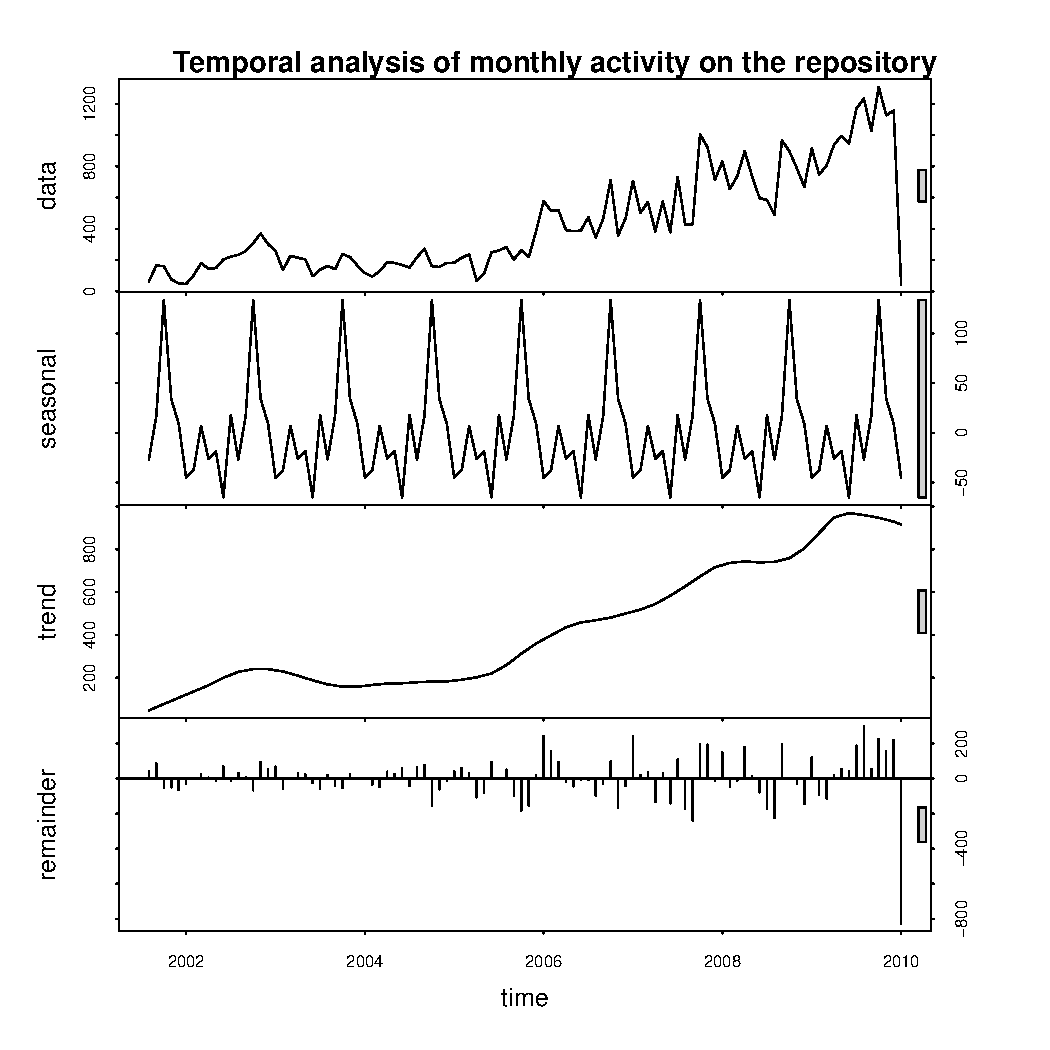
\includegraphics[width=400pt]{images/commitsByMonth.pdf}
\caption{Evolution of yearly activity in the repository}
\label{commits:evo:monthly}
\end{figure}

Figures \ref{commits:evo:weekly} and \ref{commits:evo:weekly} show the weekly and daily analysis, respectively. Together with the monthly exposed before, they show how WebKit's development model is company-led, as work load is concentrated during the office time, between monday and friday. 
Weekly analysis shows how the peak of activity is concentrated at the beginning of the week, and decreases slowly after that, with little to none work done on Saturdays and Sundays.  
Daily analysis is more interesting, as it shows how the activity increases through the day, decreases a little in the lunch break, and keeps increasing until the office time is over. Then it goes down to almost zero.
The bottom line with all of these analysis is that the project is continuously increasing its activity. 

\begin{figure}[!hptb]
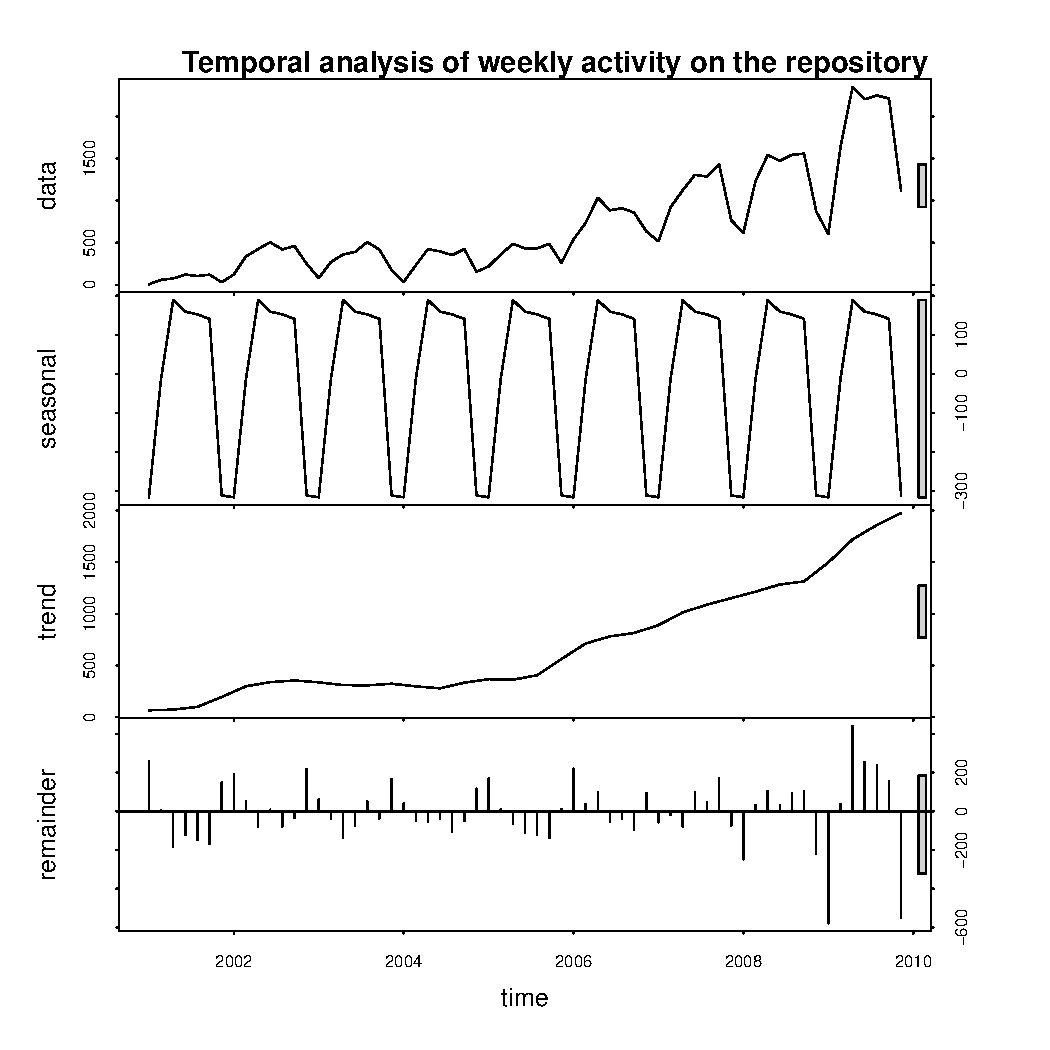
\includegraphics[width=400pt]{images/commitsByDay.pdf}
\caption{Evolution of weekly activity in the repository}
\label{commits:evo:weekly}
\end{figure}

\begin{figure}[!hptb]
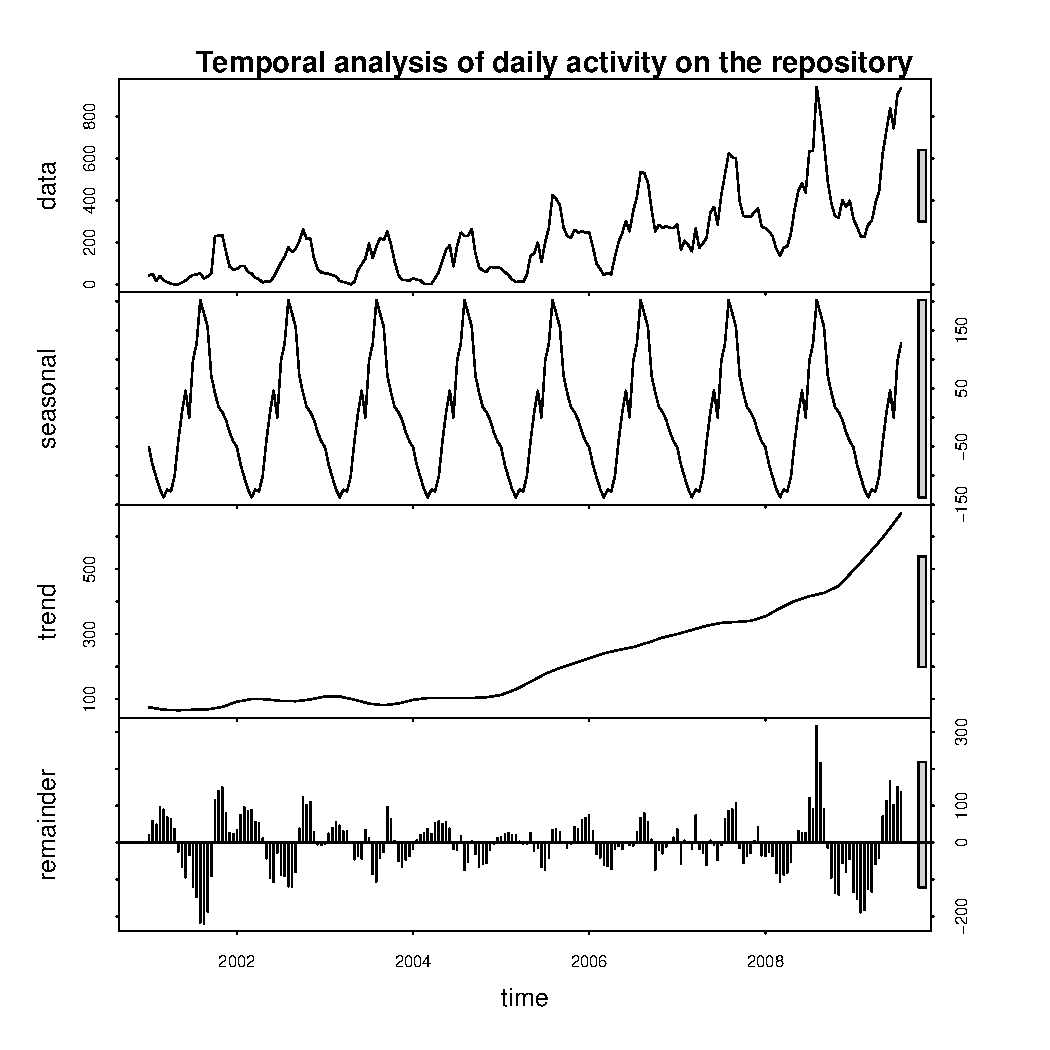
\includegraphics[width=400pt]{images/commitsByHour.pdf}
\caption{Evolution of daily activity in the repository}
\label{commits:evo:daily}
\end{figure}

In order to finish the repository analysis, figure \ref{commits:lorenz} shows the Lorenz Curve, which allows us to tell how the work is distributed among the project developers. The Gini coefficient is $0.7057624$. Those results mean that 70\% of the work is done by the 20\% of the people.

\begin{figure}[!hptb]
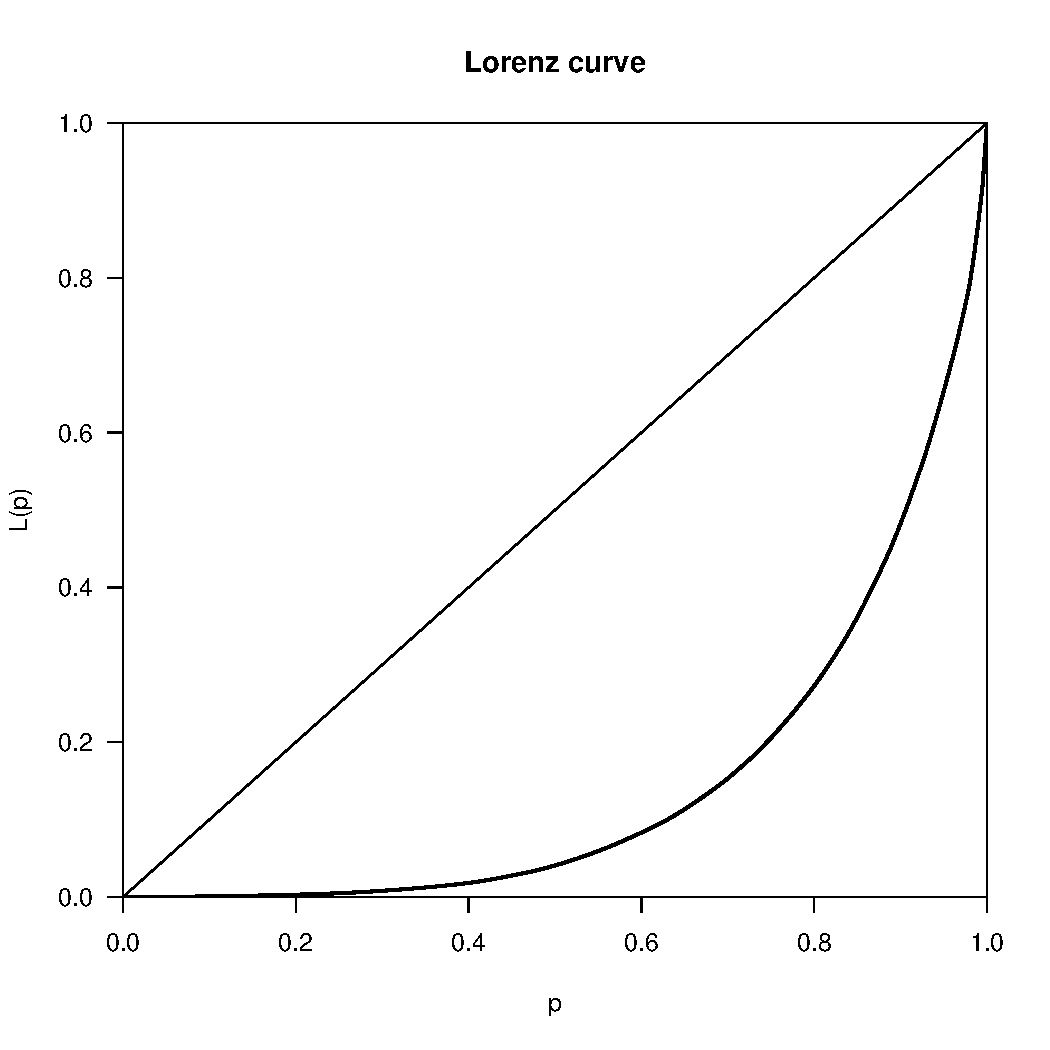
\includegraphics[width=400pt]{images/lorenz.pdf}
\caption{Lorenz curve for the repository}
\label{commits:lorenz}
\end{figure}

\subsection{Developers' mailing list}

As we did with the repository, a set of variables were taken into account to evaluate the developer's mailing list. Figure \ref{dev_mls:summary} presents the number of emails sent, number of people writing to the list and mailing list lifespan. 

\begin{table}[ht]
\begin{center}
\begin{tabular}{lr}
  \hline
Concept & Count \\ 
  \hline
Emails sent to the list & 9760 \\ 
Unique email addresses writing to the list & 1199 \\ 
Different user names writing to the list & 1132 \\
Years of activity & 5\\
   \hline
\end{tabular}
\caption{Brief summary of the developers' mailing list}
\label{dev_mls:summary}
\end{center}
\end{table}

Again, after having presented the mailing list summary, users contribution in the mailing list is measured now. Table \ref{emails:top20} shows the {\it all-time} top 20 posters to the mailing list. We can see the same user ``darin'' being the one who contributed the most, with $623$ emails sent. However, ``mjs'' is closer here, with $605$, just $18$ less than him. 

% latex table generated in R 2.9.2 by xtable 1.5-6 package
% Wed Jan 20 20:01:11 2010
\begin{table}[!htpb]
\begin{center}
\begin{tabular}{rlr}
  \hline
 & Username & Email count \\ 
  \hline
1 & darin & 623 \\ 
  2 & mjs & 605 \\ 
  3 & ddkilzer & 307 \\ 
  4 & mrowe & 209 \\ 
  5 & aroben & 206 \\ 
  6 & mike.emmel & 173 \\ 
  7 & eric & 170 \\ 
  8 & hyatt & 165 \\ 
  9 & ggaren & 160 \\ 
  10 & abarth & 147 \\ 
  11 & pkasting & 125 \\ 
  12 & bfulgham & 115 \\ 
  13 & ap & 106 \\ 
  14 & oliver & 102 \\ 
  15 & jorlow &  98 \\ 
  16 & zecke &  91 \\ 
  17 & kevino &  83 \\ 
  18 & jackwootton &  80 \\ 
  19 & jhaygood &  73 \\ 
  20 & vniles &  70 \\ 
   \hline
\end{tabular}
\caption{Top 20 posters}
\label{emails:top20}
\end{center}
\end{table}


Table \ref{emails:2009top20} shows last year's top 20 posters, so we can have current info about the mailing list. In this case, ``darin'' is still the leader with $288$ emails sent, and with ``mjs'' effectively close. If we search for ``eric'', we found him with $123$ emails sent. As he had sent $170$ in the all-time rankings, he has done $72,35\%$ of his contribution last year.

% latex table generated in R 2.9.2 by xtable 1.5-6 package
% Wed Jan 20 20:01:11 2010
\begin{table}[!htpb]
\begin{center}
\begin{tabular}{rlr}
  \hline
 & Username & Email count \\ 
  \hline
1 & darin & 288 \\ 
  2 & mjs & 233 \\ 
  3 & abarth & 132 \\ 
  4 & eric & 123 \\ 
  5 & pkasting & 106 \\ 
  6 & jorlow &  96 \\ 
  7 & ddkilzer &  86 \\ 
  8 & mrowe &  78 \\ 
  9 & ggaren &  72 \\ 
  10 & aroben &  69 \\ 
  11 & ap &  67 \\ 
  12 & atwilson &  66 \\ 
  13 & hyatt &  64 \\ 
  14 & lastguy &  61 \\ 
  15 & oliver &  54 \\ 
  16 & vniles &  54 \\ 
  17 & bfulgham &  48 \\ 
  18 & zherczeg &  48 \\ 
  19 & levin &  40 \\ 
  20 & zecke &  34 \\ 
   \hline
\end{tabular}
\caption{Top 20 posters during 2009}
\label{emails:2009top20}
\end{center}
\end{table}


As opposed to the repository, users writing to the mailing list have been sending a full email address all the time. Even if several users had more than one email address, as shown in table \ref{emails:multiple}, the queries used previously have taken it into account. 

% latex table generated in R 2.9.2 by xtable 1.5-6 package
% Wed Jan 20 20:01:11 2010
\begin{table}[!htpb]
\begin{center}
\begin{tabular}{rll}
  \hline
 & Username & Email address \\ 
  \hline
1 & aa & aa@google.com \\ 
  2 & aa & aa@chromium.org \\ 
  3 & achats & achats@avvanta.com \\ 
  4 & achats & achats@blarg.net \\ 
  5 & alex & alex@dojotoolkit.org \\ 
  6 & alex & alex@milowski.org \\ 
  7 & alex & alex@milowski.com \\ 
  8 & alex & alex@ialexi.com \\ 
  9 & alex & alex@sdpimail.com \\ 
  10 & alp & alp@atoker.com \\ 
  11 & alp & alp@nuanti.com \\ 
  12 & andersca & andersca@mac.com \\ 
  13 & andersca & andersca@apple.com \\ 
  14 & christian & christian@twotoasts.de \\ 
  15 & christian & christian@plesslweb.ch \\ 
  16 & dan & dan@dancryer.com \\ 
  17 & dan & dan@cdslash.net \\ 
  18 & danw & danw@nekotech.com \\ 
  19 & danw & danw@gnome.org \\ 
  20 & darin & darin@apple.com \\ 
  21 & darin & darin@google.com \\ 
  22 & darin & darin@chromium.org \\ 
   \hline
\end{tabular}
\caption{Email addresses for users with more than one email address}
\label{emails:multiple}
\end{center}
\end{table}
\begin{comment}
  23 & ddkilzer & ddkilzer@webkit.org \\ 
  24 & ddkilzer & ddkilzer@kilzer.net \\ 
  25 & eric & eric@puidokas.com \\ 
  26 & eric & eric@webkit.org \\ 
  27 & eric.carlson & eric.carlson@mac.com \\ 
  28 & eric.carlson & eric.carlson@apple.com \\ 
  29 & evan & evan@chromium.org \\ 
  30 & evan & evan@rainmakerinc.com \\ 
  31 & fredck & fredck@fckeditor.net \\ 
  32 & fredck & fredck@fredck.com \\ 
  33 & info & info@satzansatz.de \\ 
  34 & info & info@wake3.com \\ 
  35 & invite & invite@onlinebootycall.com \\ 
  36 & invite & invite@shopittome.com \\ 
  37 & jason & jason@jason.white.name \\ 
  38 & jason & jason@redfish.net \\ 
  39 & jcverdie & jcverdie@origyn.fr \\ 
  40 & jcverdie & jcverdie@pleyo.com \\ 
  41 & jhaygood & jhaygood@reaktix.com \\ 
  42 & jhaygood & jhaygood@spsu.edu \\ 
  43 & kevin & kevin@rhubarbproductions.com \\ 
  44 & kevin & kevin@sb.org \\ 
  45 & levin & levin@chromium.org \\ 
  46 & levin & levin@google.com \\ 
  47 & lists & lists@plenamente.com \\ 
  48 & lists & lists@roberthogan.net \\ 
  49 & lists & lists@driftbit.com \\ 
  50 & mail & mail@julianjmaurer.de \\ 
  51 & mail & mail@ruthschell.com \\ 
  52 & mark & mark@antsclimbtree.com \\ 
  53 & mark & mark@ociweb.com \\ 
  54 & mark & mark@chromium.org \\ 
  55 & martin & martin@siteloom.dk \\ 
  56 & martin & martin@gamesplace.info \\ 
  57 & martin & martin@kerz.org \\ 
  58 & martin & martin@cheetah3d.de \\ 
  59 & maruel & maruel@gmail.com \\ 
  60 & maruel & maruel@chromium.org \\ 
  61 & mbensi & mbensi@pleyo.com \\ 
  62 & mbensi & mbensi@sand-labs.com \\ 
  63 & michael & michael@tross.org \\ 
  64 & michael & michael@powerset.com \\ 
  65 & mike & mike@barrucadu.co.uk \\ 
  66 & mike & mike@maibaum.org \\ 
  67 & mike & mike@w3.org \\ 
  68 & mike & mike@softsource.com \\ 
  69 & mike & mike@belshe.com \\ 
  70 & noreply & noreply@scour.com \\ 
  71 & noreply & noreply@ci.faniq.com \\ 
  72 & opendarwin.org & opendarwin.org@mitzpettel.com \\ 
  73 & opendarwin.org & opendarwin.org@bdash.net.nz \\ 
  74 & paul & paul@zeapartners.org \\ 
  75 & paul & paul@zope-europe.org \\ 
  76 & pd & pd@opensource.dobrogost.pl \\ 
  77 & pd & pd@2009.gmane.dobrogost.pl \\ 
  78 & pkasting & pkasting@chromium.org \\ 
  79 & pkasting & pkasting@google.com \\ 
  80 & pyotel & pyotel@nate.com \\ 
  81 & pyotel & pyotel@gmail.com \\ 
  82 & rniwa & rniwa@google.com \\ 
  83 & rniwa & rniwa@webkit.org \\ 
  84 & robert & robert@ideaworks3d.com \\ 
  85 & robert & robert@elastica.com \\ 
  86 & scott & scott@eesco.com \\ 
  87 & scott & scott@realorganized.com \\ 
  88 & slightlyoff & slightlyoff@chromium.org \\ 
  89 & slightlyoff & slightlyoff@google.com \\ 
  90 & sroret & sroret@sand-labs.com \\ 
  91 & sroret & sroret@gm.sand-labs.com \\ 
  92 & sroret & sroret@origyn.fr \\ 
  93 & sroret & sroret@pleyo.com \\ 
  94 & steve & steve@opencommunity.co.uk \\ 
  95 & steve & steve@sixteenk.net \\ 
  96 & steve & steve@blighty.com \\ 
  97 & tor.arne.vestbo & tor.arne.vestbo@nokia.com \\ 
  98 & tor.arne.vestbo & tor.arne.vestbo@trolltech.com \\ 
  99 & webkit & webkit@markwang.com \\ 
  100 & webkit & webkit@propheticsky.com \\ 
  101 & webkit & webkit@blaut.biz \\ 
  102 & webkit & webkit@mattlilek.com \\ 
  103 & webkit & webkit@evpopov.com \\ 
  104 & webkit & webkit@svolli.dynxs.de \\ 
  105 & webkit & webkit@khiltd.com \\ 
  106 & webkit & webkit@different.name \\ 
  107 & webkit & webkit@kevinbroderick.com \\ 
  108 & webkit-dev & webkit-dev@joostdevalk.nl \\ 
  109 & webkit-dev & webkit-dev@ragequ.it \\ 
  110 & webkitdev & webkitdev@aol.com \\ 
  111 & webkitdev & webkitdev@gmail.com \\ 
  112 & zimmermann & zimmermann@physik.rwth-aachen.de \\ 
  113 & zimmermann & zimmermann@kde.org \\ 
\end{comment}


Thanks to the fact that it is possible to retrieve the full email address for all the project's history, the table \ref{emails:company}, which shows emails sent from a given domain address, is really interesting to see which companies supported WebKit's development. Ignoring free available domain names like ``gmail.com'' or ``yahoo.com'', Apple ({\it apple.com} and {\it webkit.org}), Google ({\it chromium.org} and {\it google.com}) or KDE ({\it kde.org}) are interesting examples about entities interested in WebKit. 

% latex table generated in R 2.9.2 by xtable 1.5-6 package
% Wed Jan 20 20:01:12 2010
\begin{table}[!htpb]
\begin{center}
\begin{tabular}{rlr}
  \hline
 & Domain name & Email count \\ 
  \hline
1 & apple.com & 2329 \\ 
  2 & gmail.com & 2244 \\ 
  3 & webkit.org & 665 \\ 
  4 & chromium.org & 423 \\ 
  5 & google.com & 337 \\ 
  6 & yahoo.com & 221 \\ 
  7 & mac.com & 169 \\ 
  8 & kde.org & 134 \\ 
  9 & kilzer.net & 110 \\ 
  10 & selfish.org &  91 \\ 
  11 & inf.u-szeged.hu &  86 \\ 
  12 & trolltech.com &  83 \\ 
  13 & theolliviers.com &  83 \\ 
  14 & nokia.com &  73 \\ 
  15 & sympatico.ca &  65 \\ 
  16 & hotmail.com &  64 \\ 
  17 & hatcher.name &  62 \\ 
  18 & atoker.com &  57 \\ 
  19 & Sun.COM &  56 \\ 
  20 & lkcl.net &  55 \\ 
   \hline
\end{tabular}
\caption{Number of emails sent by company employees}
\label{emails:company}
\end{center}
\end{table}


\subsubsection{Temporal Analysis}

Like we did with the repository, temporal analysis of the mailing list evolution through the years is a good tool to tell about WebKit's health. Again, we will present a monthly, weekly and daily analysis.

Figure \ref{mails:evo:monthly} shows how the average monthly activity evolved through the project's life. As in the repository case, there is a major peak, just before the summer time, and peaks after each holiday season. It is interesting to note how Christmas time suppose a complete halt in communications.

\begin{figure}[!hptb]
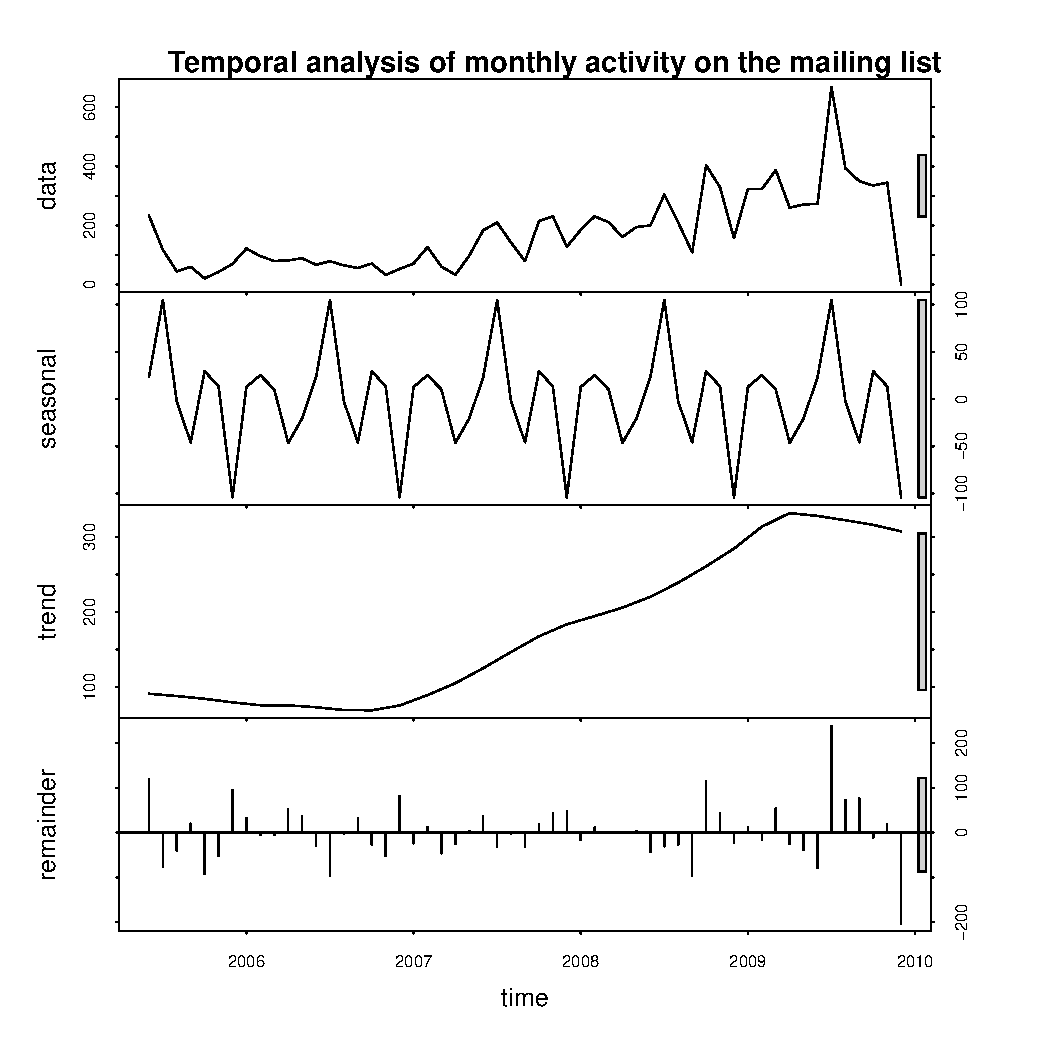
\includegraphics[width=400pt]{images/messagesByMonth.pdf}
\caption{Evolution of yearly activity in the developers' mailing list}
\label{mails:evo:monthly}
\end{figure}

Figures \ref{mails:evo:weekly} and \ref{mails:evo:weekly} show the evolution in weekly and daily activity, respectively. The weekly one shows an activity which increases through the week, going to almost-zero on Sunday. It is interesting to note that mailing list activity looks bigger than repository activity on Saturdays. Regarding to daily activity, it can be said that there is activity answering them sometime in the morning. After that, it halts around the lunch time, only to increase until the end of the office time. Surprisingly, it looks like there is another peak of activity, maybe at home now, after that break.

\begin{figure}[!hptb]
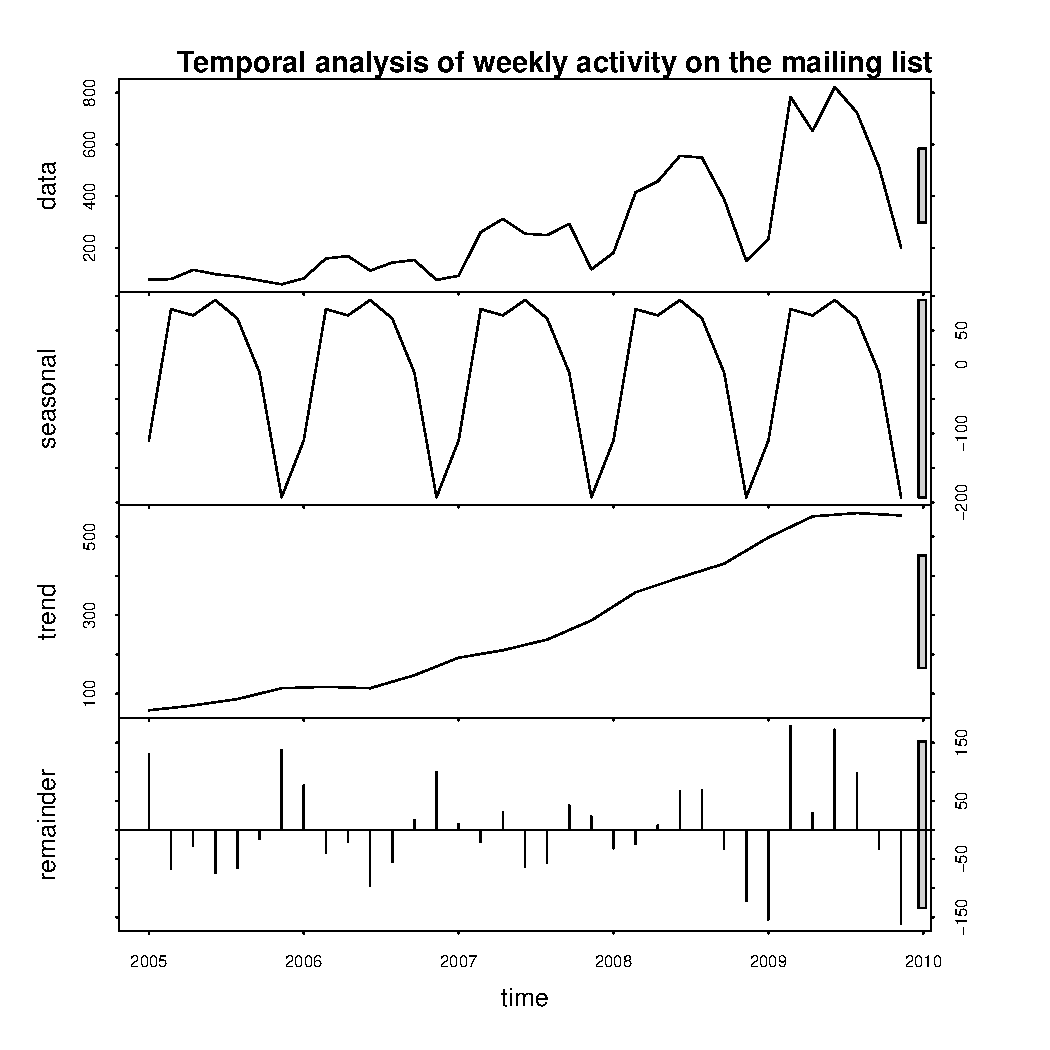
\includegraphics[width=400pt]{images/messagesByDay.pdf}
\caption{Evolution of weekly activity in the developers' mailing list}
\label{mails:evo:weekly}
\end{figure}

\begin{figure}[!hptb]
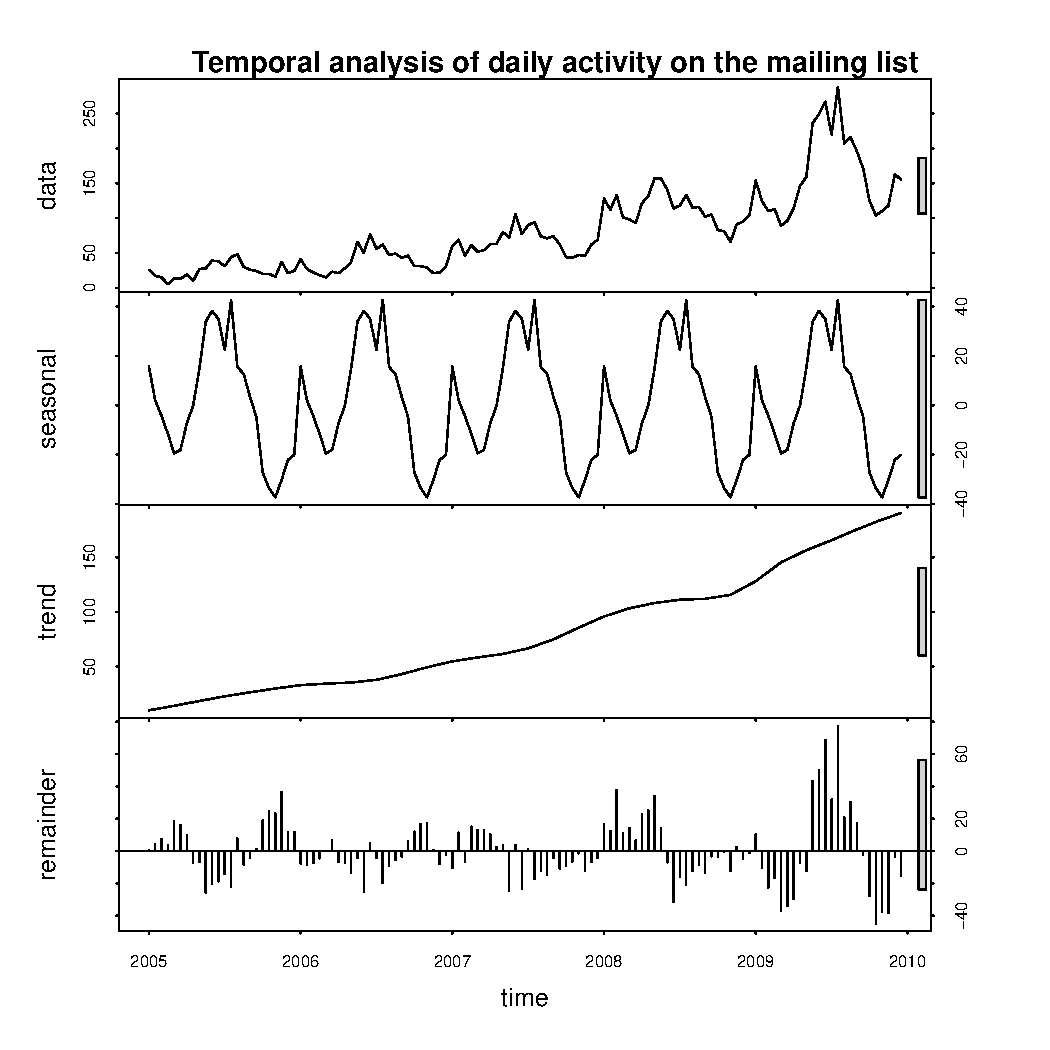
\includegraphics[width=400pt]{images/messagesByHour.pdf}
\caption{Evolution of daily activity in the developers' mailing list}
\label{mails:evo:daily}
\end{figure}

\subsection{Unassigned bugs mailing list}

Every time a bug is opened, it gets sent to this mailing list. Updates and changes regarding those bugs also send an email to the list\footnote{\url{http://webkit.org/contact.html}}. There are 160342 emails in this list. 

Figure \ref{bugs:evo:monthly} shows the average monthly activity in the mailing list. While at the beginning it has not grown as much as the developers mailing list, year 2009 seems to be a great activity explosion. Regarding to the seasonal activity, it looks like {\it bug hunting} activity also decreases during the Christmas time, just as it was professionally carried, too. After that, there is another drop in activity around February-March, and then it stays more or less constant until Christmas time again. It is interesting, as the expected drop in summer time does not appear so highlighted here.  

\begin{figure}[!hptb]
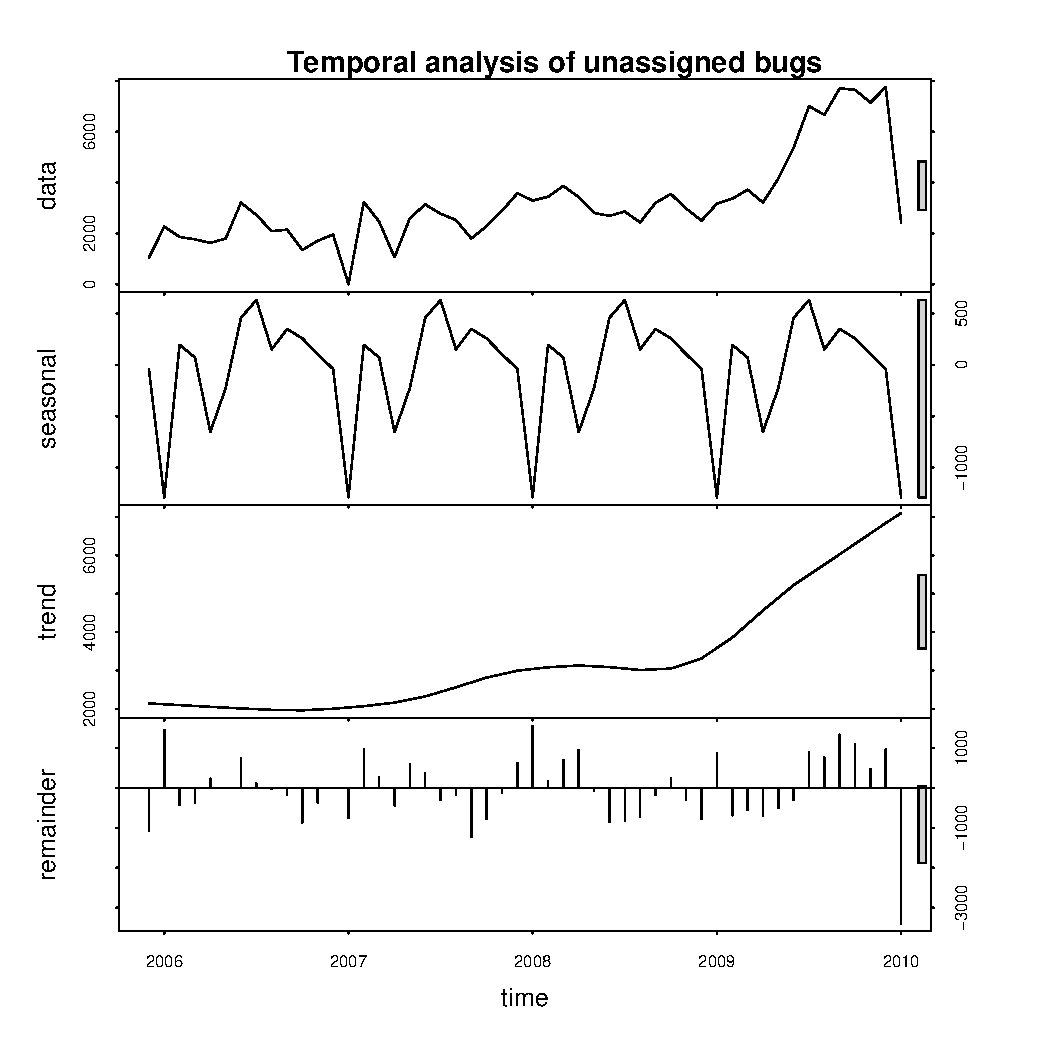
\includegraphics[width=400pt]{images/unassignedBugsByMonth.pdf}
\caption{Evolution of the monthly activity on the unassigned bugs mailing list}
\label{bugs:evo:monthly}
\end{figure}
